\documentclass{article}

\usepackage{amsmath,amssymb,scalerel,amsthm}
\usepackage[margin=0.2in]{geometry}
\usepackage{derivative}
\usepackage{mathtools}
\usepackage{color}
\usepackage{tikz}
\usetikzlibrary{arrows}


\title{Calculus II}
\author{Alessio Esposito}

\newtheorem{lemma}{Lemma}
\newtheorem{theorem}{Theorem}
\newtheorem{observation}{Obs}
\newtheorem{corollary}{Corollary}
\newtheorem{definition}{Definition}
\newtheorem{proposition}{Proposition}
\newtheorem*{schwarztheorem}{Theorem (Schwartz)}
\newtheorem*{lagrangemult}{Theorem (Lagrange Multipliers)}
\newtheorem*{implicitfunctions}{Theorem (Implicit Functions)}


\begin{document}
\maketitle

    \begin{theorem}
        $A$ is closed $\Longleftrightarrow$ every accumulation point for $A$ is in $A$ \hfill    
    \end{theorem}
    \begin{proof}
        $"\Longrightarrow"$ Let $A \subseteq \mathbb{R}^n, \ A = A \cup \partial A. \\$ Then $\forall  p \in \bar{\mathcal{D}} (A), \ C_r(p)_{\diagdown p}\cap A \neq \emptyset \ \forall  C \in \mathcal{C}_p.$ \\
        if $ p \notin A $ then $C_r(p)$ has elements that dont belong to $A \Rightarrow p \in \partial A.$ \\
        $"\Longleftarrow"$ Let $p \in \partial A \Rightarrow \forall C \in \mathcal{C}_p$ of center $r$ with $r \in \mathbb{R}$ by definition we can find some $x \in C_{\diagdown p} \cap A, $ so that means $p \in \bar{\mathcal{D}} (A) \Rightarrow p \in A.$       
    \end{proof}

\subsection*{Limits}

    \begin{definition}
        Let $A \subseteq \mathbb{R}^2$ and $(x_0,y_0)$ an accumulation point for $A.$ we define $A^*$ as follows: \\ 
        $A^* = \{(\rho , \theta) \in [0, +\infty ] \times [0, 2\pi] : (x_0 + \rho \cos(\theta), y_0 + \rho \sin(\theta)) \in A \}.$

    \end{definition}
        
    \begin{proposition}
        Lets suppose that exist a circle $C$ of center $(x_0,y_0)$ such that $C_{\diagdown \{ (x_0,y_0) \}} \subseteq A$ let $r$ be the radius of the circle and as a consequence $(0,r] \times [0,2\pi] \subseteq A^*$
    \end{proposition}
    
    \begin{proof}
        Let $C_{\diagdown \{ (x_0,y_0) \}}$ and
            $\begin{cases}
                0 < \rho \leqslant r \\
                0 \leqslant \theta \leqslant 2\pi
            \end{cases}$
            if $(\rho, \theta) \in (0,r] \times [0,2\pi]$ \\ then $(x_0 + \rho \cos(\theta), y_0 + \rho \sin(\theta)) \in C_{\diagdown \{ (x_0,y_0) \}} \subseteq A \Rightarrow (\rho, \theta) \in A^*$.
    \end{proof}
        
    \begin{definition}
        Let $\theta \in [0,2\pi]$ and $\forall \rho \in (0,r]$ we define $\varphi_\theta(\rho) = F(\rho, \theta)$ if $\rho \in (0,r], (\rho, \theta) \in A^*$ so the $\lim_{\rho \to 0} \varphi(\rho) = l \in \bar{\mathbb{R}}$. \\
        If that limit exists that means $\forall \theta \in [0, 2\pi]$ and $\forall \varepsilon > 0$, $\exists \delta > 0 \ \forall \rho \in (0,r]$ with $\rho < \delta \ \left\lvert \varphi_\theta - l \right\rvert < \varepsilon.$ \\
        We say that $\lim_{\rho \to 0} \varphi(\rho) = l \in \bar{\mathbb{R}} $ Uniformly With Respect To $(U.W.R.T.) \ \theta.$     
    \end{definition}
            
    \begin{theorem}
        Let $f:A\subseteq \mathbb{R}^2 \rightarrow \mathbb{R} $ with $(x_0,y_0)$ accumulation point for $A.$ \\ Follows the equivalence: \\ $\lim_{(x,y) \to (x_0,y_0)} f(x,y) = l \in \bar{\mathbb{R}} \Longleftrightarrow \lim_{\rho \to 0} F(\rho, \theta ) = l \ U.W.R.T. \ \theta.$ 
    \end{theorem}

    \begin{proof}
        Let $l \in \bar{\mathbb{R}}. \\$
        $"\Longrightarrow" \ \lim_{(x,y) \to (x_0, y_0)} f(x,y) = l$ so $\forall \varepsilon > 0, \exists \delta > 0: \forall \ (x,y) \in A$ \\ with $\left\lVert (x,y) - (x_0,y_0)\right\rVert < \delta, \ \left\lvert f(x,y) - l \right\rvert < \varepsilon. \\ \\$
        We have to prove that $\forall \varepsilon > 0, \ \exists \delta > 0 : \forall \theta \in [0,2\pi], \ \forall \rho (0,r] \\$ with $\rho < \delta \ \left\lvert F(\rho, \theta) - l\right\rvert < \varepsilon. \\$
        Let $\varepsilon > 0, \ \theta \in [0,2\pi], \ \rho \in (0,r]$ with $\rho < \delta.$ we create the system that changes the coordinates from cartesians to polars:
        \begin{equation*}
            \begin{cases}
                x = x_0 + \rho \cos(\theta) \\
                y = y_0 + \rho \sin(\theta) 
            \end{cases} \rho = \sqrt{(x - x_0)^2 + (y - y_0)^2} 
        \end{equation*}
        $\rho \in (0,r], \ \theta \in [0,2\pi] \in (0,r] \times [0,2\pi] \subseteq A^*, \ (\rho,\theta) \in A^* \Rightarrow (x,y) \in A. \\ \\$ 
        Now $ 0 < \sqrt{(x - x_0)^2 + (y - y_0)^2} = \rho < \delta \Rightarrow \left\lvert f(x,y) - l \right\rvert < \varepsilon. \\ $
        $\Rightarrow \left\lvert f(x_0 + \rho \cos(\theta), y_0 + \rho \sin(\theta)) - l \right\rvert < \varepsilon \Rightarrow \left\lvert F(\rho, \theta) - l \right\rvert < \varepsilon. \\ \\$
        $"\Longleftarrow" \ \forall \varepsilon > 0, \exists \delta \leq r : \forall \theta \in [0,2\pi]$ and $\forall \rho$ with $ 0 < \rho < \delta \Rightarrow \\ \left\lvert F(\rho, \theta) - l \right\rvert < \varepsilon. \\$
        We have to prove that $\forall \varepsilon > 0, \exists \delta > 0, \forall (x,y) \in A$ with \\ $ \sqrt{(x - x_0)^2 + (y - y_0)^2} = \left\lVert (x,y) - (x_0,y_0) \right\rVert  < \delta \Rightarrow \left\lvert f(x,y) - l \right\rvert < \varepsilon. \\ \\$
        Let $\varepsilon > 0, \ \delta \leq r, \ (x,y) \in A, \ \sqrt{(x - x_0)^2 + (y - y_0)^2} < \delta,$ we switch coordinates with $\rho$ and $\theta$ as follows:
            \begin{equation*}
                \begin{cases}
                    x = x_0 + \rho \cos(\theta) \\
                    y = y_0 + \rho \sin(\theta)  
                \end{cases} \rho = \sqrt{(x - x_0)^2 + (y - y_0)^2} 
            \end{equation*}
        $0< \rho < \delta \leq r \Rightarrow \rho \in (0,r), \ \theta \in [0,2\pi]. \\$ 
        We notice that $ \left\lvert F(\rho, \theta) - l \right\rvert < \varepsilon,$ so $ \left\lvert f(x_0 + \rho \cos(\theta), y_0 + \rho \sin(\theta)) - l \right\rvert < \varepsilon \\$
        $ \Rightarrow  \left\lvert f(x,y) - l \right\rvert < \varepsilon.$
    \end{proof}
    \begin{definition}
        We say that $\theta \in [0,2\pi]$ is admissible if $ 0\in \bar{\mathcal{D}}(A_\theta).$
    \end{definition}
    \begin{definition}
        Let's suppose that $\lim_{\rho \to 0} F(\rho, \theta) = l \in \mathbb{R}$ then $\forall \rho \in (0,r], \ \varphi(\rho) = \sup \left\{\left\lvert F(\rho, \theta) - l \right\rvert : \theta \in [0,2\pi]\right\} $
    \end{definition}
    \begin{theorem}
        $\lim_{\rho \to 0} F(\rho, \theta) = l \in \bar{\mathbb{R}} \ U.W.R.T. \ \theta \Longleftrightarrow \lim_{\rho \to 0 } \varphi(\rho) = 0.$
        \begin{proof}
            \textbf{($\Rightarrow$)} $\forall \varepsilon > 0 \ \exists \delta > 0 : \forall \theta \in [0,2\pi] $ and $ \forall \rho \in (0,r]$ with $\rho < \delta \ \left\lvert F(\rho, \theta) - l \right\rvert < \frac{\varepsilon}{2}$ so $\left\lvert \varphi (\rho) \right\rvert \leq \frac{\varepsilon}{2} < \varepsilon \Rightarrow \lim_{\rho \to 0} \varphi (\rho) = 0$. ($\Leftarrow$) $\forall \varepsilon > 0 \ \exists \delta > 0: \forall \rho \in (0,r)$ with $\rho < \delta \ \varphi (\rho) < \varepsilon$ but $\left\lvert F(\rho, \theta) - l \right\rvert \leq \varphi (\rho) \forall \theta$ so if $\rho \in (0,r]$ and $\rho < \delta \ \left\lvert F(\rho, \theta) - l \right\rvert < \varepsilon \Rightarrow \\ \Rightarrow \lim_{\rho \to 0} F(\rho,\theta) = l \ U.W.R.T. \ \theta$  
        \end{proof}
    \end{theorem}
    \begin{corollary}
        $\lim_{\rho \to 0} F(\rho, \theta) = l \in \bar{\mathbb{R}} \ U.W.R.T. \ \theta \Longleftrightarrow \exists$ a function $\psi(\rho)$ such that $\lim_{\rho \to 0} \psi(\rho) = 0$ and $\forall \theta \ \left\lvert F(\rho, \theta) - l\right\rvert \leqslant \psi(\rho).$
    \end{corollary}
    \begin{corollary}
        Let's suppose that $\lim_{\rho \to 0} F(\rho, \theta) = +\infty. \\ \forall \rho \in (0,r]$ let $h(\rho) = inf\{F(\rho, \theta) : \theta \in [0,2\pi] \}$ so then $\lim_{\rho \to 0} F(\rho, \theta) = +\infty \ U.W.R.T. \ \theta \Longleftrightarrow \lim_{\rho \to 0} h(\rho) = +\infty $
    \end{corollary}
    \begin{observation}
        $\lim_{\rho \to 0} F(\rho, \theta) = +\infty \ U.W.R.T. \ \theta \Longleftrightarrow \exists$ a function $K(\rho) \ s.t. \\ \lim_{\rho \to 0}K(\rho) = +\infty$ and $F(\rho,\theta) \geq K(\rho)$ 
    \end{observation}
    \begin{corollary}
        Let's suppose that $\lim_{\rho \to 0} F(\rho, \theta) = -\infty. \\ \forall \rho \in (0,r]$ let $g(\rho) = sup\{F(\rho, \theta) : \theta \in [0,2\pi] \}$ so then $\lim_{\rho \to 0} F(\rho, \theta) = -\infty \ U.W.R.T. \ \theta \Longleftrightarrow \lim_{\rho \to 0} g(\rho) = -\infty$
    \end{corollary}
    \begin{definition}
        Let $f : A \subseteq \mathbb{R}^2 \rightarrow \mathbb{R}$ with $A$ open.\\
        let $(x_0,y_0) \in A$, $\varphi(x) = f(x,y_0)$ and $\psi = f(x_0,y)$.
        $A$ is open that means that those two functions are well defined. 
    \end{definition}
    \subsection*{Differentiability}
    \begin{definition}
        Let be $f : A \subseteq \mathbb{R}^n \rightarrow \mathbb{R}$ with $A$ Open.
        Let $\bar{x} \in A$ and let $i \leq n$, we denote as $\varphi_i(x_i) = f(\bar{x}_1, \bar{x}_2, ... ,\bar{x}_{i-1},\bar{x}_i, \bar{x}_{i+1}, ... , \bar{x}_n)$. \
        Notice that $\bar{x}$ is an internal point so then it exist an interval where $\varphi_i$ is well defined. 
    \end{definition}
    \begin{definition}
        We say that $f$ is partially derivable with respect to the variable $x_i$ in the point $\bar{x}$ if $\varphi_i$ is derivable in that point.
        We denote as $\frac{\partial f}{\partial x_i}$ the partial derivative with respsect to $x_i$ in the point $\bar{x}$. 
    \end{definition}
    \begin{definition}
        The gradient of a function in $n$ variables is defined as follows:
        \begin{equation*}
            \nabla f : \bar{x} \in A \longmapsto  \left( \frac{\partial f}{\partial x_1},..., \frac{\partial f}{\partial x_n} \right)  \in \mathbb{R}^n
        \end{equation*}
    \end{definition}
    Let $f : A \subseteq \mathbb{R}^2 \rightarrow \mathbb{R}$ with $A$ open, and let $(x_0,y_0) \in A$. \\ $(x_0,y_0, f(x_0,y_0)) \in \mathcal{G}(f)$. The equation of the plane that passes for \\ $(x_0,y_0, f(x_0,y_0))$ is $Z = f(x_0,y_0) + a(X-x_0) + b(Y-y_0)$ where $a,b \in \mathbb{R}$.
    \begin{definition}
        We say that $f$ is partially derivable with respect to $x$ in $(x_0,y_0)$ if $\varphi$ is differentiable in $x_0$.
        in that case we $\varphi$ is the partial derivative of $f$ in the variable $x$ and its written $\frac{\partial f}{\partial x}$ 
    \end{definition}
    \begin{definition}
        We define the gradient as $\nabla f : (x,y) \in A \longmapsto \left( \frac{\partial f}{\partial x},\frac{\partial f}{\partial y} \right) \in \mathbb{R}^2$
    \end{definition}
    \begin{definition}
        We say that $f$ is differentiable in the point $(x_0, y_0)$ if exists $a,b \in \mathbb{R}$ such that:
        \begin{equation*}
            \lim_{(x, y) \to (x_0,y_0)} \frac{f(x,y)-f(x_0,y_0)-a(X-x_0)-b(Y-y_0)}{\left\lVert (x,y) - (x_0,y_0)\right\rVert } = 0  \ (\vartriangle) 
        \end{equation*}
        f is differentiable in the point $(x_0,y_0)$ if exists a plane that passes in the point $(x_0,y_0, f(x_0,y_0))$ that approximates the graph of the function $f$.
        \begin{proposition}
            If $f$ is differentiable in the point $(x_0,y_0)$, $f$ is partially derivable with respsect to $x$ and $y$ such that $a = \frac{\partial f(x_0,y_0)}{ \partial x}$ and $b = \frac{\partial f(x_0,y_0)}{ \partial y}$  
        \end{proposition}
        \begin{definition}
            if $f$ is differentiable in a point $(x,y) \in A$, the differential in the point is defined as follows:
            \begin{gather*}
                d_{(x,y)}f:(h,k) \in \mathbb{R}^2 \longmapsto \frac{\partial f(x,y)}{\partial x}h + \frac{\partial f(x,y)}{\partial y}k \in \mathbb{R}
            \end{gather*}
        \end{definition}
        \begin{definition}
            More in general if $f:A \subseteq \mathbb{R}^n \rightarrow \mathbb{R}$ and \textbf{x} $\in A$:
            \begin{equation*}
                d_{\textbf{x}}^rf:h \in \mathbb{R}^n \longmapsto \sum_{\substack{i_1, \dots, i_n \geqslant 0 \\ i_1 + \dots + i_n = r}}\frac{r!}{i_1! \dots i_n!}\frac{\partial ^r f}{\partial x^{i_1} \dots \partial x^{i_n}}(\textbf{x}) h^{i_1}_1, \dots,h^{i_n}_n  \in \mathbb{R}
            \end{equation*}
        \end{definition}
        \begin{corollary}
            $f$ is differentiable in the point $(x_0,y_0) \Longleftrightarrow f$ is partially derivable in the point $(x_0,y_0)$ and the $(\vartriangle)$ is true.
        \end{corollary}
    \newpage
        \begin{definition}
            Let $f:A \subseteq \mathbb{R}^2 \rightarrow \mathbb{R}$ with $A$ open and $k> 0$ a positive integer. let $(x_0,y_0) \in A$ and if $f$ has differentiable derivatives of order $k - 1$ we define the "k-grade Taylor polinomia" as follows:
            \begin{equation*}
                P_k(x,y) = f(x_0,y_0) + \sum_{i = 1}^{k} \frac{1}{i!}d_{(x_0,y_0)}^if(x-x_0,y-y_0)  
            \end{equation*}  
        \end{definition}
        \begin{theorem}
            Let $f : A \subseteq \mathbb{R}^2 \rightarrow \mathbb{R}$ with $A$. If $\exists \ \frac{\partial f}{\partial x}$ and $\frac{\partial f}{\partial y}$ in $A$ and are continuos in a point $(x_0,y_0)$, then the function is differentiable in $(x_0,y_0)$.
            \begin{proof}
                We have to prove that:
                \begin{equation*}
                    \lim_{(x,y) \to (x_0,y_0)}\frac{f(x,y) - f(x_0,y_0) - \frac{\partial f(x_0,y_0)}{\partial x}(x-x_0) - \frac{\partial f(x_0,y_0)}{\partial y}(y-y_0)}{\sqrt{(x-x_0)^2 + (y-y_0)^2}} = 0
                \end{equation*}
                Lets add and subtract $f(x,y_0)$, so one has:
                \begin{equation*}
                    f(x,y) - f(x_0,y_0) = f(x,y) - f(x,y_0) + f(x,y_0) - f(x_0,y_0)
                \end{equation*} 
                We call $\varphi (t) = f(x,t)$ where $t \in I[y,y_0]$ and $I[y,y_0] = \begin{cases}
                    [y,y_0] \ y \leq y_0 \\
                    [y_0,y] \ y_0 \leq y
                \end{cases}$ \\
                $\varphi$ is derivable and for the Lagrange theorem $\exists y_1 \in I[y,y_0] : \varphi (y) - \varphi (y_0) = \dot{\varphi}(y_1)(y-y_0)$. So one has $f(x,y) - f(x,y_0) = \frac{\partial f(x,y_1)}{\partial y}(y-y_0)$, and we repeat the same reasoning for the other variable and one will have $f(x,y_0) - f(x_0,y_0) = \frac{\partial f(x_1,y_0)}{\partial x}(x-x_0)$
                We have then: 
                    \begin{gather*}
                        \left\lvert \frac{f(x,y) - f(x_0,y_0) - \frac{\partial f(x_0,y_0)}{\partial x}(x-x_0) - \frac{\partial f(x_0,y_0)}{\partial y}(y-y_0)}{\sqrt{(x-x_0)^2 + (y-y_0)^2}} \right\rvert = \\ = \left\lvert \frac{\frac{\partial f(x_1,y_0)}{\partial x}(x-x_0) - \frac{\partial f(x,y_1)}{\partial y}{(y-y_0) - \frac{\partial f(x_0,y_0)}{\partial x}(x-x_0) - \frac{\partial f(x_0,y_0)}{\partial y}(y-y_0)}}{\sqrt{(x-x_0)^2 + (y-y_0)^2}} \right\rvert = \\ = \left\lvert \frac{\left(\frac{\partial f (x_1,y_0)}{\partial x} - \frac{\partial f (x_0,y_0)}{\partial x} \right)(x-x_0) + \left( \frac{\partial f (x,y_1)}{\partial x} - \frac{\partial f(x_0,y_0)}{\partial x}\right)(y-y_0)}{\sqrt{(x-x_0)^2 + (y-y_0)^2}}\right\rvert  
                    \end{gather*}
                The last member is increased by the following:
                    \begin{gather*}
                        \left\lvert \frac{\partial f(x_1,y_0)}{\partial x} - \frac{\partial f(x_0,y_0)}{\partial x} \right\rvert \frac{\left\lvert x - x_0\right\rvert}{\left\lVert (x-x_0,y-y_0)\right\rVert } + \left\lvert \frac{\partial f(x,y_1)}{\partial y} - \frac{\partial f(x_0,y_0)}{\partial y}\right\rvert \frac{\left\lvert y - y_0\right\rvert}{\left\lVert (x-x_0,y-y_0) \right\rVert } \leq \\ \leq \left\lvert \frac{\partial f(x_1,y_0)}{\partial x} - \frac{\partial f(x_0,y_0)}{\partial x} \right\rvert + \left\lvert \frac{\partial f(x,y_1)}{\partial y} - \frac{\partial f(x_0,y_0)}{\partial y}\right\rvert
                    \end{gather*}
                And since $x \to x_0 \Rightarrow x_1 \to x_0$ and $y \to y_1 \Rightarrow y_1 \to y_0$ so the second member of the inequality is equal to zero.
            \end{proof}
        \end{theorem}
    \end{definition}
    \begin{theorem} %$\left( \diamondsuit \right)$ 
        Let $f : A \subseteq \mathbb{R}^n \rightarrow \mathbb{R}$ with $A$ open. If the function is differentiable in a point \textbf{x} $\in A$ then is continuos in that point.
        \begin{proof}
            Since we have:
            \begin{equation*}
                \lim_{x \to \textbf{x}}\frac{f(x) - f(\textbf{x}) - \sum_{i = 1}^{n} \frac{\partial f(\textbf{x})}{\partial x_i} \left(x_i - \textbf{x}_i \right)}{\left\lVert x - \textbf{x}\right\rVert} = 0
            \end{equation*}
            If we fix an $\varepsilon = 1$ there exists $\delta > 0 : \forall x \in A$ with $0 < \left\lVert x - \textbf{x} \right\rVert < \delta$ one has:
            \begin{equation*}
                \left\lvert \frac{f(x) - f(\textbf{x}) - \nabla f(\textbf{x})(x - \textbf{x})}{\left\lVert x - \textbf{x}\right\rVert} \right\rvert < \varepsilon \Longrightarrow \left\lvert f(x) - f(\textbf{x}) - \nabla f(\textbf{x})(x - \textbf{x}) \right\rvert < \left\lVert x - \textbf{x}\right\rVert
            \end{equation*}
            So we have the the following:
            \begin{equation*}
                \left\lvert f(x) - f(\textbf{x}) \right\rvert - \left\lvert \nabla f(\textbf{x})(x - \textbf{x}) \right\rvert \leq \left\lvert f(x) - f(\textbf{x}) - \nabla f(\textbf{x})(x - \textbf{x}) \right\rvert < \left\lVert x - \textbf{x}\right\rVert \ \bigtriangleup 
            \end{equation*}
            The $\bigtriangleup$ implies that $\left\lvert f(x) - f(\textbf{x}) \right\rvert - \left\lvert \nabla f(\textbf{x})(x - \textbf{x}) \right\rvert \leq \left\lvert \nabla f(\textbf{x})(x - \textbf{x}) \right\rvert + \left\lVert x - \textbf{x} \right\rVert \leq \left\lVert \nabla f(\textbf{x})\right\rVert \left\lVert x - \textbf{x} \right\rVert + \left\lVert x - \textbf{x} \right\rVert$. The last member of the inequality is equal to $\left\lVert x - \textbf{x} \right\rVert\left( \nabla f(\textbf{x}) + 1 \right)\vartriangle  $  so, if $ 0 < \left\lVert x - \textbf{x} \right\rVert < \delta$ then by calling the $\vartriangle = c$ one finally has:
            \begin{equation*}
                0 < \left\lvert f(x) - f(\textbf{x}) \right\rvert \leq c\left\lVert x - \textbf{x}\right\rVert \to 0 \Leftarrow x \to \textbf{x} \Rightarrow \left\lvert f(x) - f(\textbf{x}) \right\rvert \to 0
            \end{equation*}
            Or equivalently: $\lim_{x \to \textbf{x}}f(x) = f(\textbf{x})$.
        \end{proof}
    \end{theorem}
    \newpage
    \begin{schwarztheorem}
        \footnote{$\Omega$ this time is used instead of $A$} Let $f:\Omega \subseteq \mathbb{R}^2 \rightarrow \mathbb{R}$ be a function in two variables defined on a open set $\Omega$. \\ If $f$ admits continuous second derivatives in the point ($f \in C^2(\Omega)$) then $\frac{\partial ^2 f}{\partial x \partial y} = \frac{\partial ^2 f}{\partial y \partial x}$.
        \begin{proof}
            Let $p = (x_0,y_0) \in \Omega$ and chose two real numbers $\varepsilon,\delta > 0$ such that $(x_0 - \varepsilon, x_0 + \delta) \times (y_0 - \delta, y_0 + \delta) \subset \Omega$. That is possible since $\Omega$ is Open.
            Lets also define the two functions $F$ and $G$ as follows: 
            \begin{flalign*}
                F: (-\varepsilon,\varepsilon) \subset \mathbb{R} \rightarrow \mathbb{R} \\
                G: (-\delta,\delta) \subset \mathbb{R} \rightarrow \mathbb{R}
            \end{flalign*}
            In the way that:
            \begin{flalign*}
                F(t) = f(x_0 + t, y_0 + s) - f(x_0 + t,y_0) \ \ \forall s \in (- \delta, \delta) \\
                G(s) = f(x_0 + t, y_0 + s) - f(x_0,y_0 + s) \ \ \forall t \in (-\varepsilon, \varepsilon)
            \end{flalign*}
            It can be easily proved that: $F(t) - F(0) = G(s) - G(0)$ also if we apply the Lagrange theorem two times one has: $F(t) - F(0) = t\Dot{F}(\xi_1)$ with $t\Dot{F}(\xi_1)$ equal to: $t \left[ \frac{\partial f}{\partial x}(x_0 + \xi_1, y_0 + s) - \frac{\partial f}{\partial x}(x_0 + \xi_1,y_0) \right] = ts\frac{\partial ^2 f}{\partial y \partial x}(x_0 + \xi_1, y_0 + \sigma_1)$. The same reasoning can be applied to $G(s) - G(0)$ obtaining: $st\frac{\partial ^2 f}{\partial x \partial y}(x_0 + \xi_2, y_0 + \sigma_2)$ with $\xi_i \in (0,t)$ and $\sigma_i \in (0,s)$ where without loss of generality we can say $t,s > 0$. \\
            Thinking about $t \rightarrow 0$ and $s \rightarrow 0 \Rightarrow \xi_i \rightarrow 0$ and $\sigma_i \rightarrow 0$ with the continuity of the two derivatives one has: $\frac{ \partial ^2 f}{\partial y \partial x}(x_0,y_0) = \frac{ \partial ^2 f}{\partial x \partial y}(x_0,y_0)$.
        \end{proof}
    \end{schwarztheorem}
    \subsection*{Directional Derivatives}
    If we take $f : A \subseteq \mathbb{R}^2 \rightarrow \mathbb{R}$ defined on an open set $A$, $(x_0,y_0) \in A$ and a vector of unitary norm $\vec{v} = (v_1,v_2)$, the Directional derivative of $f(x_0,y_0)$ along the direction $\bar{v}$ can be defined as the limit if it exists and its finite:
    \begin{equation*}
        \frac{\partial f}{\partial \bar{v}}(x_0,y_0) = \lim_{t \to 0} \frac{f(x_0 + tv_1, y_0 + tv_2) - f(x_0,y_0) }{t}
    \end{equation*}
    \subsection*{Study of the maxima and minima}
        \begin{definition}
            If a partial derivative $\frac{\partial f}{\partial x}$ of a function $f : A \subseteq \mathbb{R}^2 \rightarrow \mathbb{R}$ is partially derivable with respect to $x$ in a point $(x_0,y_0) \in A$ we say that $f$ is partially derivable two times with respect to $x$ in the point $(x_0,y_0)$ ad it will be denoted as $\frac{\partial f}{\partial x}f_x(x_0,y_0)=\frac{\partial^2 f(x_0,y_0)}{\partial x^2} = \frac{\partial^2 f}{\partial x^2}(x_0,y_0)$. \\
            The same goes for the other partial derivatives: $\frac{\partial}{\partial y}f_x = \frac{\partial^2 f}{\partial x \partial y}$, $\frac{\partial}{\partial x}f_y = \frac{\partial^2 f}{\partial y \partial x}, \ldots $            
        \end{definition}
        \begin{definition}
            We define the hessian matrix as follows:
        \begin{equation*}
            \mathcal{D}^2f = \left(\begin{matrix}
                \frac{\partial^2 f}{\partial x^2} & \frac{\partial ^2 f}{\partial x \partial y} \\ \frac{\partial^2 f}{\partial y \partial x} & \frac{\partial ^2 f}{\partial y^2} 
            \end{matrix} \right)  
        \end{equation*}
        \end{definition}
        \begin{definition}
            The determinant of $\mathcal{D}^2f$ is: 
            \begin{equation*}
                \mathcal{H}(x,y) = \left\lvert \begin{matrix}
                \frac{\partial^2 f}{\partial x^2} & \frac{\partial ^2 f}{\partial x \partial y} \\ \frac{\partial^2 f}{\partial y \partial x} & \frac{\partial ^2 f}{\partial y^2} 
            \end{matrix} \right\rvert 
        \end{equation*} and is called the Hessian determinant.
        \end{definition}
        \begin{definition}
            Let $f : A \subseteq \mathbb{R}^2 \rightarrow \mathbb{R}$, we say that $(x_0,y_0) \in A$ is maxima (minima) for $f$ if $\forall (x,y) \in A, \ f(x,y) \leqslant f(x_0,y_0)$ \ ($f(x,y) \geqslant f(x_0,y_0)$). 
        \end{definition}
        \begin{theorem}
            If $f$ is continuous and $A$ is compact, $f$ admits minima and maxima.
        \end{theorem}
        \begin{theorem}
            Let $f : A \subseteq \mathbb{R}^2 \rightarrow \mathbb{R}$ and let $(x_0,y_0) \in \dot{A}$ a relative extreme and let  $f$ be partially derivable in $(x_0,y_0)$, so then $\frac{\partial f(x_0,y_0)}{\partial x} = 0$ and $\frac{\partial f(x_0,y_0)}{\partial y} = 0$. \\
            The points where the partial derivatives are $0$ are said "critical points" of $f$, $(x_0,y_0) \in \dot{A}$ is an extreme ralative $\Rightarrow$ $(x_0,y_0)$ is a critical point for $f$ ($\nLeftarrow$).         
        \end{theorem}
        \begin{observation}
            Let $(x_0,y_0) \in A$ and let $g(x,y) = f(x,y) - f(x_0,y_0)$, $(x_0,y_0)$ is a relative minimum (relative maximum) for $f \Longleftrightarrow \ \exists$ a circle $C$ of center $(x_0,y_0)$ such that $g \geq 0$ ($g \leq 0$).
        \end{observation}
        \begin{theorem}
            Let $f : A \subseteq \mathbb{R}^2 \rightarrow \mathbb{R}$ and let $(x_0,y_0) \in \dot{A}$ a relative extreme $\Longrightarrow \mathcal{H}(x_0,y_0) \geqslant 0$.
        \end{theorem}
        \begin{theorem}
            Let $f : A \subseteq \mathbb{R}^2 \rightarrow \mathbb{R}$, $f \in \mathbf{C}^2$. Let $(x_0,y_0) \in \dot{A}$ a critical point and lets suppose that $\mathcal{H}(x_0,y_0) > 0 \Longrightarrow (x_0,y_0)$ is a relative extreme and is maximum or minimum depending on $\frac{\partial^2 f(x_0,y_0)}{\partial x^2}$ be $<0$ or $>0$.  
        \end{theorem}
        \newpage
        \subsection*{Vectorial Functions}
            A vectorial function is defined as follows: $f:A \subseteq \mathbb{R}^n \rightarrow \mathbb{R}^m$. $\forall x \in A, \ f(x) \in  \mathbb{R}^m$ and $f(x) = (f_1(x),\dots,f_m(x))$ with $f_i:A \subseteq \mathbb{R}^n \rightarrow \mathbb{R}$
            \begin{definition}
                Let $f:A \subseteq \mathbb{R}^n \rightarrow \mathbb{R}^m$ and let $x_0$ be an accumulation point for $A$, we say that $\lim_{x \to x_0}f(x) = l \in \mathbb{R}^m$ if $\forall \varepsilon >0 \ \exists \delta > 0: \forall x\in A$ with $0 < \left\lVert x - x_0 \right\rVert < \delta \Rightarrow \left\lVert f(x) - l\right\rVert < \varepsilon $.
            \end{definition}
            \begin{lemma}
                Let $a_1,\dots,a_n \in \mathbb{R}$, then $\forall j \leq n \ \left\lvert a_j \right\rvert \leq \sqrt{\sum_{i = 1}^{n}a_i^2} \leq \sum_{i = 1}^{n}\left\lvert a_i \right\rvert$.
                \begin{proof}
                    Let $j \leq n$. $\left\lvert a_j \right\rvert = \sqrt{a_j^2} \leq \sqrt{\sum_{i = 1}^{n} a_i^2 }$. We have to prove that $\sum_{i = 1}^{n} a_i^2 \leq \left( \sum_{i = 1}^{n}\left\lvert a_i \right\rvert \right)^2 $  and thats true for $n = 2$ infact: $\left(\left\lvert a_1 \right\rvert + \left\lvert a_2 \right\rvert  \right)^2 = a_1^2 + a_2^2 + 2\left\lvert a_1 \right\rvert\left\lvert a_2 \right\rvert \geq a_1^2 + a_2^2$. Lets suppose that's true for $n - 1$, that means $\sum_{i = 1}^{n}a_i^2 \leq \left(\sum_{i = 1}^{n}\left\lvert a_i \right\rvert\right)^2$ because $\sum_{i = 1}^{n}a_i^2  = \sum_{i = 1}^{n-1}a_i^2 + a_n^2 \leq \left(\sum_{i = 1}^{n - 1}\left\lvert a_i \right\rvert\right)^2 + a_n^2 \leq \left(\sum_{i = 1}^{n - 1}\left\lvert a_i \right\rvert + \left\lvert a_n \right\rvert \right)^2 = \left(\sum_{i = 1}^{n}\left\lvert a_i \right\rvert\right)^2$.      
                \end{proof}
            \end{lemma}
            \begin{theorem}
                Let $f:A\subseteq \mathbb{R}^2 \rightarrow \mathbb{R}^m$ with $f=(f_1,\dots,f_m)$. Let $x_0$ be an accumulation point for $A$ and let $l = (l_1,\dots,l_m) \in \mathbb{R}^m$. Then $\lim_{x \to x_0}f(x) = l \Longleftrightarrow  \forall i \leq m, \ \lim_{x \to x_0}f_i = l_i$.
                \begin{proof}
                    We know that if $a_i = f_i(x) - l_i$ then $\forall j \leq m, \ \left\lvert f_j(x) - l_j\right\rvert \leq \sqrt{\sum_{i = 1}^{m} \left(f_i(x) - l_i\right)^2 } = \left\lVert f(x) - l\right\rVert \leq \sum_{i = 1}^{m} \left\lvert f_i(x) - l_i\right\rvert$. Lets suppose that $\lim_{x \to x_0} f(x) = l$, then $\left\lVert f(x) - l\right\rVert \to 0 $ for $x \to x_0$ and for the sandwich theorem $\left\lvert f_j (x) - l_j \right\rvert \to 0 $ for $x \to x_0 \ \forall j \leq m \Longrightarrow \forall j \leq m \ \lim_{x \to x_0 }f_j(x) = l_j$. Viceversa lets suppose that $\forall i \leq m \ \lim_{x \to x_0} f_i( x) = l_i \Rightarrow \left\lvert f_i (x) - l_i\right\rvert \to 0 $ for $x \to x_0 \forall i \leq m \Rightarrow \ \sum_{i = 1}^{m} \to 0$ for $x \to x_0 \ \Rightarrow \left\lVert f(x) - l\right\rVert \to 0 $ for $x \to x_0 \Rightarrow \lim_{x \to x_0}f(x) = l$.  
                \end{proof}
            \end{theorem}
            \begin{definition}
                $f(x)$ is continuous in a point $x_0 \in A$ if $\forall \varepsilon > 0, \exists \delta$ such that $\forall x \in A,  \left\lVert x - x_0\right\rVert < \delta \Rightarrow \left\lVert f(x) - f(x_0) \right\rVert < \varepsilon$.
            \end{definition}
            \begin{proposition}
                If $x_0$ is an isolated point, $f$ is continuous in $x_0$. If $x_0$ is an accumulation point, $f$ is continuous in $ x_0 \Longleftrightarrow \lim_{x \to x_0} f(x) = f(x_0) \Longleftrightarrow \forall i \leq m \ \lim_{x \to x_0} f_i(x) = f_i(x_0)$.   
            \end{proposition}
            \begin{corollary}
                $f$ is continuous $\Longleftrightarrow$ all its components are continuous.
            \end{corollary}
            \begin{definition}
                $f: A \subseteq \mathbb{R}^n \rightarrow \mathbb{R}^m$ with A open. We say that $f$ is partially derivable with respect to the variable $x_i$ in a point $\overline{x} \in A$ if it exists:
                \begin{equation*}
                    \lim_{x \to \overline{x_i}} \frac{f(\overline{x_1},\dots,x_i,\dots,\overline{x_n}) - f(\overline{x})}{x_i - \overline{x_i}} \in \mathbb{R}^m
                \end{equation*} 
            \end{definition}
            \begin{theorem}
                Let $f = (f_1,\dots,f_m)$. Then $f$ is partially derivable with respect to $x_j$ in the point $\overline{x} \in A \Longleftrightarrow \forall i \leq m \ f_i$ is partially derivable with respect to $x_j$ in the point $\overline{x}$. Also $\frac{\partial f}{\partial x_j} = \left( \frac{\partial f_1}{\partial x_j},\dots,\frac{\partial f_m}{\partial x_j}\right)$.
                \begin{proof}
                    $\lim_{x \to \overline{x_i}} \frac{f(\overline{x_1},\dots,x_i,\dots,\overline{x_n}) - f(\overline{x})}{x_i - \overline{x_i}}$. The $i-$component of the incremental ratio is $\lim_{x \to \overline{x_j}} \frac{f_i(\overline{x_1},\dots,x_j,\dots,\overline{x_n}) - f_i(\overline{x})}{x_j - \overline{x_j}}$. \\ 
                    $\lim_{x \to \overline{x_i}} \frac{f(\overline{x_1},\dots,x_i,\dots,\overline{x_n}) - f(\overline{x})}{x_i - \overline{x_i}}$ exists $\Longleftrightarrow \forall i \leq m$ exists $\lim_{x \to \overline{x_j}} \frac{f_i(\overline{x_1},\dots,x_j,\dots,\overline{x_n}) - f_i(\overline{x})}{x_j - \overline{x_j}} \Longrightarrow f$ is partially derivable with respect to $x_j$ in the point $\overline{x} \Longleftrightarrow$ all its components are derivable.
                \end{proof}
            \end{theorem}
            \begin{definition}
                If $f:A \subseteq \mathbb{R}^n \rightarrow \mathbb{R}^m$ is partially derivable with respect to all variables, we define:
                \begin{equation*}
                    \nabla f : x \longmapsto \left( \begin{matrix}
                        \frac{\partial f_1}{\partial x_1} (x) && \dots && \frac{\partial f_1}{\partial x_n}(x) \\
                        \vdots && \ddots  && \vdots \\
                        \frac{\partial f_m}{\partial x_1} (x) && \dots && \frac{\partial f_m}{\partial x_n}(x) \\
                    \end{matrix}\right) \ \diamondsuit
                \end{equation*}
                As the Jacobian matrix. The $\diamondsuit$ can be also written as $\nabla f = \frac{\partial \left(f_1, \dots, f_m\right) }{\partial \left(x_1,\dots, x_n\right)}$. If $m = n$ the Jacobian matrix is a square matrix and the determinant is called Jacobian determinant.
            \end{definition}
            \begin{lemma}
                If $h \in \mathbb{R}^n$ the prodouct rows for coloumns $\nabla f(x) \cdot h \in \mathbb{R}^m$ and has for components $\nabla f_i \cdot h$. $\nabla f(x) \cdot h = \left(\nabla f_1 \cdot h, \dots, \nabla f_m \cdot h\right)$
                \begin{proof}
                    $\nabla f(x)$ is a $m \times n$ matrix. If $h \in \mathbb{R}^n$ then it can be written as a $n \times 1$ matrix, so $\forall x \in A, \ \nabla f(x) \cdot h$ is a $m \times 1$ matrix therefore an element of $\mathbb{R}^m $.  $h = \left( \begin{matrix} h_1 \\ \vdots \\ h_n \end{matrix} \right) \Longrightarrow \nabla f(x) \cdot h = \left( \frac{\partial f_1}{\partial x_1}(x)h_1 + \dots + \frac{\partial f_1}{\partial x_n}(x)h_n, \dots, \frac{\partial f_m}{\partial x_1}(x)h_1 + \dots + \frac{\partial f_m}{\partial x_n}(x)h_n\right)$.
                \end{proof}
            \end{lemma}
            \begin{definition}
                We say that $f$ is differentiable in a point $x \in A$ if is partially derivable with respect to all the variables in the point $x$ and:
                \begin{equation*}
                    \lim_{h \to 0 } \frac{f(x +h) - f(x)- \nabla f(x) \cdot h}{\left\lVert h \right\rVert}
                \end{equation*}
                Is equal to zero.
            \end{definition}
            \newpage
        \subsection*{Implicit functions}
            By defining a function $f:A \subseteq \mathbb{R}^2 \rightarrow \mathbb{R}$ the expression: $f(x,y) = 0 \ \Diamond  $ means that one can consider the variable $x$ as a parameter and $y$ as unknown and the question is when, $\forall x \ \exists! y$ such that the $\Diamond $ is true.  
            \begin{definition}
                The equation defines implicitly $y$ as a function of $x$ if $\forall x, \exists! y: f(x,y) = 0$ in that case the function g is defined as:
                \begin{equation*}
                    g:x \longmapsto y \Rightarrow f(x,y) = 0
                \end{equation*}
            \end{definition}
            \begin{proposition}
                The equation $f(x_0,y_0) = 0$ defines implicitly $y$ as a function of $x$, the set of all the zeros of $f$ is equal to the graph of the implicit function.
                \begin{proof}
                    $(x_0,y_0)$ is a zero of $f \Longleftrightarrow f(x_0,y_0) = 0 \Longleftrightarrow y_0 = g(x_0) \Longleftrightarrow (x_0,y_0) \in Gr(g)$
                \end{proof}
            \end{proposition}
            \begin{implicitfunctions}
                Let $f:A \subseteq \mathbb{R}^2 \rightarrow \mathbb{R}$ lets suppose that $f$ and $\frac{\partial f}{\partial y}$ are continuous. Let $(x_0,y_0) \in A$ be a zero of of the function where $\frac{\partial f}{\partial y} (x_0,y_0) \neq 0$. \textbf{i.} Then there exists an open interval $I$ of center $x_0$ and an open interval $J$ of center $y_0 : I \times J \subseteq A$ and $\forall x \in I, \ \exists! y \in J : f(x,y) = 0$. \textbf{ii.} Also if $g: I \rightarrow J$ is the implicit function, $g$ is continuous and $g(x_0) = y_0$. \textbf{iii.} In addition if $\exists \frac{\partial f}{\partial x}, \ g$ is derivable and $\forall x \in I, \ \dot{g}(x) = -\frac{\frac{\partial f}{\partial x}(x,g(x))}{\frac{\partial f}{\partial y}(x,g(x))}$. \textbf{iv.} Furthermore $f \in C^k$, then $g\in C^k$.  
                \begin{proof}
                    \textbf{i.} By hypotesis $\frac{\partial f}{\partial y} \neq 0$. Lets suppose that $\frac{\partial f}{\partial y}(x_0,y_0) > 0$, so for the sign permanence theorem there exists a rectangle $R_0 = [x_0 - \alpha , x_0 + \alpha] \times [y_0 - \beta , y_0 + \beta] \subseteq A : \forall (x,y) \in R_0, \ \frac{\partial f}{\partial y}(x,y) > 0$. Let $\varphi: y\in [y_0 - \beta , y_0 + \beta] \longmapsto f(x_0,y)$, by hypotesis $\exists \frac{\partial f}{\partial y}$ so, by definition $\varphi$ is derivable and $\dot{\varphi}(y)= \frac{\partial f}{\partial y}(x_0,y) > 0 \Rightarrow \varphi$ is strictly growing. $\varphi (y_0) = f(x_0,y_0) = 0, \ \varphi (y_0 + b) > \varphi(y_0) = 0 \Rightarrow f(x_0,y_0 - b) < 0$ and $f(x_0,y_0+b) > 0$. Lets define:
                    \begin{gather*}
                        \varphi_1: x\in [x_0- \alpha,x_0 + \alpha] \longmapsto f(x,y_0 - b) \\
                        \varphi_2: x\in [x_0- \alpha,x_0 + \alpha] \longmapsto f(x,y_0 + b)
                    \end{gather*}
                    $\varphi_1$ and $\varphi_2$ are continuous because $f$ is continuous and $\varphi_1 (x_0) = f(x_0,y_0 -b) < 0$ and $\varphi_2(x_0) = f(x_0,y_0 + b) > 0$ so there exists an interval $[x_0 - \delta, x_0 + \delta] \subseteq [x_0 - \alpha, x_0 + \alpha] : \forall x \in [x_0 - \delta, x_0 +\delta], \ \varphi_1(x) < 0$ and $\varphi_2(x) > 0$. Now $\forall x \in [x_0 - \delta, x_0 +\delta], f(x,y_0 - b) < 0 $ and $f(x,y_0 + b ) > 0$ if we take an $x \in (x_0 - \delta, x_0 +\delta)$ and define: 
                    \begin{equation*}
                        \psi: y\in [y_0 - b, y_0 + b] \longmapsto f(x,y)
                    \end{equation*}
                    One has that $\psi$ is derivable and $\dot{\psi}(y) = \frac{\partial f}{\partial y}(x,y) >0$ that implies $\psi$ is strictly growing and also continuous. $\psi (y_0 - b) = f(x,y_0 - b) < 0$ and $\psi(y_0 + b) = f(x,y_0 + b) > 0$ for the zeros theorem, $\exists y \in (y_0 - b, y_0 + b)$ where $\psi(y) = 0 \Rightarrow f(x,y) = 0$. Also $y$ is unique since $\psi$ is strictly growing and that means it can't become zero in two diffrent points.
                    \textbf{ii.} Let $g: I \longmapsto J$ the implicit function defined by the equation $f(x,y) = 0$. $\forall x \in I, \ f(x,g(x)) = 0$ and $f(x_0,y_0) \Rightarrow y_0 = g(x_0)$ we have to prove that $g$ is continuous, so let $\overline{x} \in I$ and the claim is $\lim_{x \to \overline{x}}g(x) = g(\overline{x})$. $\forall x \in I, \ g(x)$ and $g(\overline{x})$ are two distinct points of $J \Rightarrow K[g(x),g(\overline{x})] \subseteq J$. \\
                    \begin{center} 
                        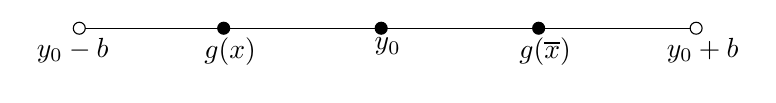
\begin{tikzpicture}
                            \draw [o-*] (0,0) node[pos = 1, below] {$y_0 - b$} -- +(2,0) node[pos = 1, below] {$g(x)$};
                            \draw [-*] (2,0) -- +(2,0) node[pos = 1, below] {$y_0$}; 
                            \draw [-*] (2,0) -- +(4,0) node[pos = 1, below] {$g(\overline{x})$};
                            \draw [-o] (4,0) -- +(4,0) node[pos = 1, below] {$y_0 + b$};
                        \end{tikzpicture}
                    \end{center}   
                    $\forall x \in I$, let $\psi : y\in K[g(x),g(\overline{x})] \longmapsto f(x,y)$ 
                    with $\dot{\psi}(y) = \frac{\partial f}{\partial y}(x,y) > 0$, for the lagrange theorem, $\exists$ a point $\xi_x \in K[g(x),g(\overline{x})]:$ 
                    \begin{gather*}
                        \psi(g(x)) - \psi(g(\overline{x})) = \dot{\psi}(\xi_x)(g(x) - g(\overline{x})) 
                    \end{gather*}
                    That becomes: $f(x,g(x)) - f(x,g(\overline{x})) = \frac{\partial f}{\partial y}(x,\xi_x)(g(x) - g(\overline{x})) \Rightarrow g(x) - g(\overline{x}) = -\frac{f(x,g(\overline{x}))}{\frac{\partial f}{\partial y}(x,\xi_x)} \Rightarrow \left\lvert g(x) - g(\overline{x}) \right\rvert = \frac{\left\lvert f(x,g(\overline{x})) \right\rvert }{\left\lvert \frac{\partial f}{\partial y}(x,\xi_x)\right\rvert}$.
                    $\frac{\partial f}{\partial y}$ is continuous and $R_0$ is compact. By the Weierstrass theorem there exists $m = \min\left\{ \left\lvert \frac{\partial f}{\partial y} (x,y) \right\rvert : (x,y) \in R_0 \right\}$, $\frac{\partial f}{\partial y} > 0$ in $R_0$ and that means $m > 0$ so $\left\lvert \frac{\partial f}{\partial y} (x,y) \right\rvert \geq m$ therefore one has:
                    \begin{equation*}
                        \left\lvert g(x) - g(\overline{x}) \right\rvert = \frac{\left\lvert f(x,g(\overline{x}))\right\rvert }{\frac{\partial f}{\partial y}(x,\xi_x)} \leq \frac{f(x,g(\overline{x}))}{m}    
                    \end{equation*}
                    $x \to \overline{x} \Rightarrow (x,g(\overline{x})) \to (\overline{x},g(\overline{x})), \ f$ is continuous $\Rightarrow f(x,g(\overline{x})) \to f(\overline{x},g(\overline{x})) = 0 $ so $\lim_{x \to \overline{x}}g(x) = g(\overline{x})$. \textbf{iii.} Let $\overline{x} \in I$ we have to prove that $g$ is derivable in $\overline{x}$. If $x \in I$ 
                    \begin{equation*} 
                        g(x) - g(\overline{x}) = - \frac{f(x,g(\overline{x}))}{\frac{\partial f}{\partial y}(x,\xi_x)} \Rightarrow \frac{g(x) - g(\overline{x})}{x - \overline{x}} = -\frac{1}{\frac{\partial f}{\partial y}(x,\xi_x)}\frac{f(x,g(\overline{x})) - f(\overline{x},g(\overline{x}))}{x - \overline{x}} \ \blacktriangle    
                    \end{equation*}
                    And since there exists the partial derivative of $f$ with respsect to $x$ the last member of the $\blacktriangle$ is the incremental ratio of the function $f(x,g(\overline{x}))$ in the point $f(\overline{x},g(\overline{x}))$ and by examining $\frac{\partial f}{\partial y}(x,\xi_x)$ with $\xi_x \in K[g(x) - g(\overline{x})], \ x \to \overline{x} \Rightarrow g(x) \to g(\overline{x}) \Rightarrow \xi_x \to g(\overline{x}) \Rightarrow (x,\xi_x) \to (\overline{x}, g(\overline{x}))$. $\frac{\partial f}{\partial y}$ is continuous $\Rightarrow \lim_{x \to \overline{x}} \frac{\partial f}{\partial y}(x, \xi_x) = \frac{\partial f}{\partial y}(\overline{x},g(\overline{x}))$ finally $\exists \lim_{x \to \overline{x}}\frac{g(x) - g(\overline{x})}{x - \overline{x}} = -\frac{\frac{\partial f}{\partial x}(\overline{x},g(\overline{x}))}{\frac{\partial f}{\partial y}(\overline{x},g(\overline{x}))}$. \textbf{iv.} is proved by induction infact, if we take $k = 1$ if $f \in C^1$ its partial derivatives are continuous so $g$ is continuous, the rest can be easily verified.
                \end{proof}

            \end{implicitfunctions}
        \subsection*{Bound extremes}
        Let $f: A \subseteq \mathbb{R}^n \rightarrow \mathbb{R}$ with $A$ open. If $g: A \rightarrow \mathbb{R}^m$ then we define $E_0 = \left\{ x\in A: g(x) = 0 \right\}$. $g = (g_1 ,\dots ,g_m)$ so $g(x) = 0$ is equivalent to say:        
        \begin{equation*}
            \begin{cases}
                g_1(x) = 0 \\
                g_2(x) = 0 \\
                \vdots \\
                g_m(x) = 0
            \end{cases}
        \end{equation*}
        \begin{definition}
            A point  $x_0 \in E_0$ is said to be bound maximum (bound minimum) if $\forall x \in E_0 \ f(x) \leq f(x_0)$ ($f(x) \geq f(x_0)$).
        \end{definition}
        \begin{lagrangemult}
            Let $f:A\subseteq \mathbb{R}^2 \rightarrow \mathbb{R}$ and $g:A \rightarrow \mathbb{R}$ with $g \in C^1$ in an open set $A$. \\ 
            Let $E_0 = \left\{ (x,y)\in A: g(x,y)= 0 \right\}$ and $(x_0,y_0) \in E_0$ a bound relative extreme for $f$ and suppose that $\nabla g(x_0,y_0) \neq (0,0)$ then $\exists ! \lambda \in \mathbb{R} : (x_0,y_0)$ be a critical point for the function $\mathcal{L} (x,y) = f(x,y) + \lambda g(x,y)$ $\left( \frac{\partial f}{\partial x}(x_0,y_0) + \lambda \frac{\partial g}{\partial x}(x_0,y_0) = 0 \land \frac{\partial f}{\partial y}(x_0,y_0) + \lambda \frac{\partial g}{\partial y}(x_0,y_0) = 0\right)$.
            \begin{proof}
                \textbf{Existence} Since $\nabla g(x_0,y_0) \neq (0,0)$ we can assume $\frac{\partial g}{\partial y}(x_0,y_0) \neq 0$. $g(x,y) = 0$ verifies the conditions of the implicit functions theorem ($g \in C^1, \ g(x_0,y_0) = 0, \ \frac{\partial g}{\partial y}(x_0,y_0) \neq 0$), so for that theorem $\exists$ an open interval $I$ of center $x_0$ and an open interval $J$ of center $y_0: I \times J \subseteq A$ and $\forall x \in I \ \exists ! \ y \in J: g(x,y)=0$ also the implicit function $\varphi : I \rightarrow J$ is $C^1$. $\varphi (x_0) = y_0$ and $\forall x \in I$ one has: 
                \begin{equation*}
                    \dot{\varphi}(x) = - \frac{\frac{\partial g}{\partial x}(x, \varphi (x))}{\frac{\partial g}{\partial y}(x, \varphi (x))}
                \end{equation*} 
                Lets suppose for example that $(x_0,y_0)$ is a bound relative maximum, then there exists a rectangle $I' \times J' \subseteq I \times J$ of center $(x_0,y_0)$ such that $\forall (x,y) \in (I'\times J')\cap E_0 \Rightarrow f(x,y) \leq f(x_0,y_0)$. $\varphi$ is continuous in $x_0$, $J'$ is an interval of center $y_0 = \varphi(x_0) \ \exists  I'' \subseteq I'$ of center $x_0 : \forall x \in I'' \ \varphi(x) \in J'$. $\forall x \in I'' \ (x,\varphi(x)) \in (I' \times J') \cap E_0$. $\varphi :x \longmapsto$ y such that $g(x_0,y_0) = 0$ so $g(x,\varphi(x)) = 0 \ \forall x \in I$. $\forall x \in I'' \ f(x,\varphi(x)) \leq f(x_0,y_0)$. $\forall x \in I''$ we define $\psi(x) = f(x,\varphi(x))$ such that $\forall x \in I''$ we have $(x,\varphi(x)) \in I' \times J' \subseteq I\times J \subseteq A$ and that means $\forall x \ \psi(x) \leq f(x_0,y_0) = \psi(x_0) \Rightarrow x_0$ is a bound relative maximum for $\psi$ and is internal to $I''$. $\psi \in C^1$ since is a composition of $C^1$ functions so is derivable and $\forall x \in I''$:
                \begin{equation*}
                    \dot{\psi}(x) = \frac{\partial f}{\partial x}(x,\varphi (x)) + \frac{\partial f}{\partial y}(x,\varphi (x)) \dot{\varphi} (x) = \frac{\partial f}{\partial x}(x,\varphi (x)) - \frac{\partial f}{\partial y}(x,\varphi (x)) \frac{\frac{\partial g}{\partial x}(x,\varphi (x))}{\frac{\partial g}{\partial y}(x,\varphi (x))}
                \end{equation*}
                Since $\psi$ is derivable, and $x_0$ is a maximum, for fermat theorem one has $\dot{\psi}(x_0)=0$ with: 
                \begin{equation*}
                    \dot{\psi}(x_0) = \frac{\partial f}{\partial x}(x_0,y_0) - \frac{\partial f}{\partial y}(x_0,y_0) \frac{\frac{\partial g}{\partial x}(x_0,y_0)}{\frac{\partial g}{\partial y}(x_0,y_0)} = 0 \Longleftrightarrow  \frac{\partial f}{\partial x}(x_0,y_0)\frac{\partial g}{\partial y}(x_0,y_0) - \frac{\partial f}{\partial y}(x_0,y_0)\frac{\partial g}{\partial x}(x_0,y_0) = 0
                \end{equation*}
                Equivalently we can use this expression:
                \begin{equation*}
                    \begin{vmatrix}
                        \frac{\partial f}{\partial x}(x_0,y_0) && \frac{\partial f}{\partial y}(x_0,y_0) \\
                        \frac{\partial g}{\partial x}(x_0,y_0) && \frac{\partial g}{\partial y}(x_0,y_0)
                    \end{vmatrix} = 0
                \end{equation*}
                And if thats is true that implies $\exists (\lambda_1, \lambda_2) \neq (0,0)$ such that one of the two coloums is \textbf{l.d.} \footnote{Linearly dependent} $\Longrightarrow \lambda_1\frac{\partial f}{\partial x}(x_0,y_0) + \lambda_2\frac{\partial g}{\partial x}(x_0,y_0) = 0$. \\
                If $\lambda_1 = 0 \Rightarrow \lambda_2 \neq 0 \Rightarrow \frac{\partial g}{\partial x}(x_0,y_0) = 0$ but that's impossible since the hypotesis impose it to be different from zero, so it must be $\lambda_1 \neq 0$ and if we chose $\lambda = \frac{\lambda_2}{\lambda_1}$ we have $\mathcal{L} (x,y) = f(x,y) + \lambda g(x,y) = 0$. \\
                \textbf{Uniqueness} Let $\mathcal{L} (x,y) = f(x,y) + \lambda g(x,y) = 0$ and $\mathcal{L} (x,y) = f(x,y) + \overline{\lambda}  g(x,y) = 0$. If we subtract member to member the last equations one has: 
                \begin{equation*}
                    \left( \lambda - \overline{\lambda} \right) \frac{\partial g}{\partial y}(x_0,y_0) = 0 \Rightarrow  \lambda = \overline{\lambda}
                \end{equation*}
            \end{proof} 
        \end{lagrangemult}
\end{document}